\documentclass[letterpaper,10pt]{article}

\usepackage{titling}
\usepackage{listings}
\usepackage{url}
\usepackage{setspace}
\usepackage{subfig}
\usepackage{sectsty}
\usepackage{pdfpages}
\usepackage{colortbl}
\usepackage{multirow}
\usepackage{multicol}
\usepackage{relsize}
\usepackage{amsmath}
\usepackage{fancyvrb}
\usepackage[yyyymmdd]{datetime}
\usepackage{amsmath,amssymb,amsthm,graphicx,xspace}
\usepackage[titlenotnumbered,noend,noline]{algorithm2e}
\usepackage[compact]{titlesec}
\usepackage{XCharter}
\usepackage[T1]{fontenc}
\usepackage{tikz}
\usetikzlibrary{arrows,automata,shapes,trees,matrix,chains,scopes,positioning,calc}
\tikzstyle{block} = [rectangle, draw, fill=blue!20, 
    text width=2.5em, text centered, rounded corners, minimum height=2em]
\tikzstyle{bw} = [rectangle, draw, fill=blue!20, 
    text width=4em, text centered, rounded corners, minimum height=2em]

\definecolor{namerow}{cmyk}{.40,.40,.40,.40}
\definecolor{namecol}{cmyk}{.40,.40,.40,.40}
\renewcommand{\dateseparator}{-}


\let\LaTeXtitle\title
\renewcommand{\title}[1]{\LaTeXtitle{\textsf{#1}}}


\newcommand{\handout}[5]{
  \noindent
  \begin{center}
  \framebox{
    \vbox{
      \hbox to 5.78in { {\bf ECE252: Systems Programming and Concurrency } \hfill #2 }
      \vspace{4mm}
      \hbox to 5.78in { {\Large \hfill #4  \hfill} }
      \vspace{2mm}
      \hbox to 5.78in { {\em #3 \hfill \today } }
    }
  }
  \end{center}
  \vspace*{4mm}
}

\newcommand{\lecture}[3]{\handout{#1}{#2}{#3}{Lecture #1}}{
\newcommand{\tuple}[1]{\ensuremath{\left\langle #1 \right\rangle}\xspace}

\addtolength{\oddsidemargin}{-1.000in}
\addtolength{\evensidemargin}{-0.500in}
\addtolength{\textwidth}{2.0in}
\addtolength{\topmargin}{-1.000in}
\addtolength{\textheight}{1.75in}
\addtolength{\parskip}{\baselineskip}
\setlength{\parindent}{0in}
\renewcommand{\baselinestretch}{1.5}
\newcommand{\term}{Spring 2019}

\singlespace


\begin{document}

\lecture{ 6 --- Processes in UNIX}{\term}{Jeff Zarnett}

\section*{The Process in UNIX}

Earlier on, we saw that in UNIX, a process may create other processes. The creating process is the parent and the newly-created processes are its children. Every process has a parent, stretching back to the \texttt{init} process at the root of the tree.

Each process has a unique identifier in its process control block, and in UNIX we call this the \texttt{pid} (process ID). For the most part, users will not need to know or think about the ID of a process except when trying to terminate one that's gotten stuck (\texttt{kill -9 24601}). The \texttt{init} process always gets a pid of 1. I don't recommend trying to kill \texttt{init}. In most cases, \texttt{init} will just laugh off your attempt (``'tis but a scratch!'') but you might end up rebooting the system or causing a crash.

\begin{center}
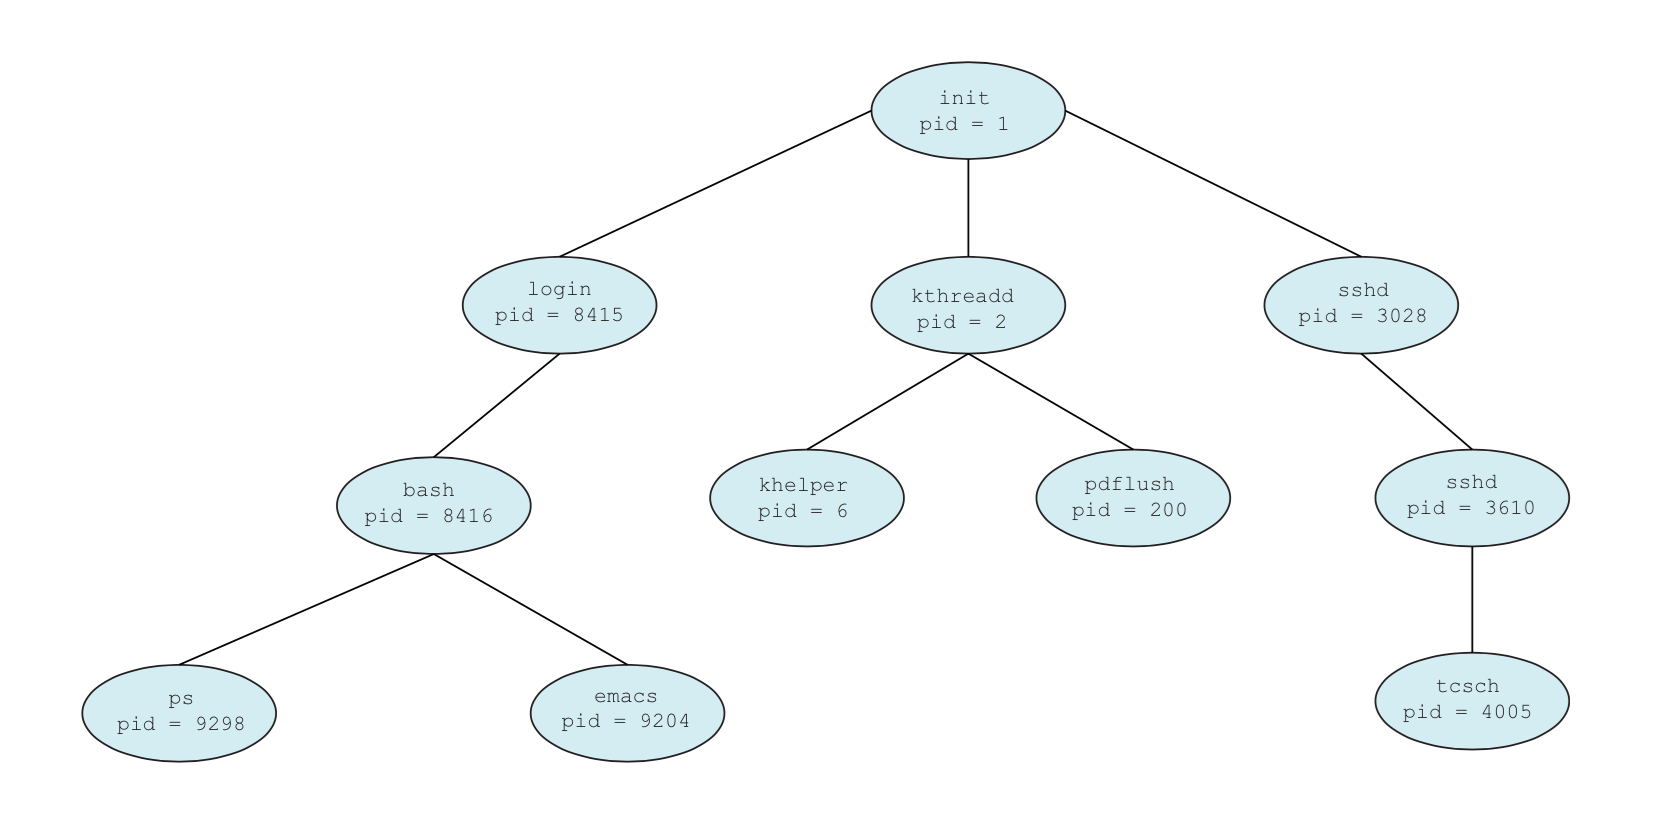
\includegraphics[width=0.5\textwidth]{images/linux-process-tree.png}\\
A tree of processes in a Linux system~\cite{osc} \footnote{...one of whose authors apparently uses \texttt{emacs} instead of \texttt{vi}. Shame on him.}.
\end{center}

In a UNIX system, we can obtain a list of processes at any time with the \texttt{ps} command. The diagram illustrates that each user, when logging in, spawns a \texttt{login} process (and an administrator can log people out by killing their \texttt{login} process... not that this is necessarily a good way to do it). The user's shell (these days, almost always \texttt{bash}, the Bourne Again Shell) is then spawned from \texttt{login}. That shell provides the command line interface where the user can enter a command.

When you issue a command, like \texttt{ls} or \texttt{top} (table of processes), the new process is created and the shell will \texttt{wait} on that process to finish (in the case of \texttt{ls}) or for the user to tell it to exit (\texttt{top}); when it does, control goes back to the shell and you get presented with the prompt again (e.g., \texttt{jz@Loki:\~{}/\$}). This would, on its face, seem kind of limiting -- do I have to log in to the system in a second terminal window to run two things at a time? The answer is no, and there are two ways to get around it.

The first thing we can do is tell the shell we want the task to run in the background. To do that, add to the command the \texttt{\&} symbol, like so: 

\texttt{gcc fork.c \&}

This will return control almost immediately to the shell (as it will not be waiting for the \texttt{gcc} command to finish). You may see some output like \texttt{[1] 34429} which is the shell saying the child has been created and it has process ID 34429. When the process is finished, there is another update, looking something like:

\texttt{[1]+  Done                    gcc fork.c}

Notably, any console output that the \texttt{gcc} command would generate will still appear on the console where the background task was created. Maybe you want that but maybe you want to put the output in a log file, with a command like \texttt{cat fork.c > logfile.txt \&}. (Telling \texttt{gcc} to be silent is a somewhat more complex operation.) The semantics of \texttt{\&} are not just saying ``run this in the background, please''; it is actually the parent process (the shell) disowning its child (the \texttt{cat} or \texttt{gcc} process) so that process will get adopted by \texttt{init} and can run to completion even if the user logs out.

A common example of a command I use involving the \texttt{\&}:\\
\texttt{ sudo service xyz start \& }\\
This will (with super user permissions - that's the purpose of \texttt{sudo}) start up the service \texttt{xyz} but return control to the console so I don't have to wait for the \texttt{xyz} service to be started to enter my next command. This is good, because the next thing I'd like to do is \texttt{tail -f /var/log/xyz/console.log} which will allow me to watch the console log of the \texttt{xyz} service as it starts up to see if there are any errors.

The other alternative to get something to run in the background is with the \texttt{screen} command. While having something run in the background is nice, it does not work for interactive processes. Suppose you are working on some code in \texttt{vi} and you would like to pause that for a minute and write an e-mail (with \texttt{pine} or whatever the cool kids use for command line e-mail these days). One approach is to save and exit \texttt{vi} and open up \texttt{pine}. The other would be to start up each of these in \texttt{screen} and switch between them. 

Thus instead of just opening \texttt{vi fork.c} I can issue the command \texttt{screen vi fork.c} and this spawns \texttt{screen} and takes me right to editing the file. The key difference is that I can ``detach'' from this screen and go back to the command line that spawned it. And if I log out, \texttt{screen} keeps running with the \texttt{vi} inside it. If I have multiple screens running, I can just ``reattach'' to the one I want to use next. To get a full understanding of \texttt{screen}, try the command \texttt{man screen} and the user manual will appear to give you some information and instructions about how to use this. Or you can use Google. 

\subsection*{Spawning Child Processes}

In general, when a process spawns a child, the child will need resources (memory, files etc.). The child may request them from the OS directly or the parent can give some of its resources to the child. The parent may partition resources amongst the children or allow its children to share them instead. Restricting a child process to only being able to use some subset of its parent's resources means that a process cannot overload the system by spawning too many children~\cite{osc}.

At the time of initialization, the parent may pass the child some data. When the user clicks on a link in an e-mail\footnote{Remember when I said don't do this? I meant it.} and the e-mail client spawns the web browser, the browser doesn't just open a blank page or the user's normal home page; instead it starts up with the address the user just clicked on.

When a new process is created, the child process may be a duplicate of the parent process, or it may have a new program loaded into it.


\subsection*{Show Me The Code!}

The workflow in UNIX is as follows. First, the parent spawns the child process with the \texttt{fork} system call. If it is interested in waiting for the child process to finish, it will use the system call \texttt{wait}, in which case the parent will be awaiting the completion of the child process. When the child process is finished, it returns a value with the \texttt{exit} system call. The parent process will then get this as the return value of the \texttt{wait} call and may proceed.

What does \texttt{fork} do? It creates a new process; it makes a copy of itself. The parent and child continue execution after the \texttt{fork} statement. If \texttt{fork} returns a negative number, the \texttt{fork} system call failed. If it returns 0, the process that got the 0 back is the child. If it returns a positive value, that is the process ID of the child.

After the \texttt{fork}, one of the processes may use the \texttt{exec} system call, or one of its variants, to replace its memory space with a new program. There's no rule that says this must happen; a child can continue to be a clone of its parent if it wishes. The \texttt{exec} invocation loads the binary file into memory and starts execution~\cite{osc}. At this point, the programs can go their separate ways, or the parent might want to wait for the child to finish. The parent is then blocked, waiting for the child process to execute.

Let's put this all together in an actual C-code example adapted from~\cite{osc}:

\begin{verbatim}
#include <sys/types.h>
#include <stdio.h> 
#include <unistd.h>

int main()
{
  pid_t pid;
  int childStatus;

  /* fork a child process */
  pid = fork();
  
  if (pid < 0) { 
  
    /* error occurred */ 
    fprintf(stderr, "Fork Failed"); 
    return 1;
    
 } else if (pid == 0) { 
    
    /* child process */
    execlp("/bin/ls","ls",NULL);
    
  } else { 
    
    /* parent process */
    /* parent will wait for the child to complete */
    wait(&childStatus);
    printf("Child Complete with status: %i \n", childStatus);
    
  }
    
  return 0;
}
\end{verbatim}

When executed, this code starts up and attempts to spawn a child process. Let us assume that the \texttt{fork} command succeeds and we do not enter the error-occurred block.  After the fork there are now two processes at the statement \texttt{ if ( pid < 0 ) } . The child process calls \texttt{execlp}, replacing itself with the \texttt{ls} (list directory contents) command. The parent process will go to the \texttt{wait} statement and wait for the child process to complete. The child process runs \texttt{ls}, listing the contents of the directory. Then it finishes. The parent process, finally, prints ``Child Complete'' to the console.

Thus, the output is:
\begin{verbatim}
jz@Freyja:~/fork$ ./fork 
fork   fork.c
Child Complete with status: 0
jz@Freyja:~/fork$ 
\end{verbatim}

Or, to represent this visually:

\begin{center}
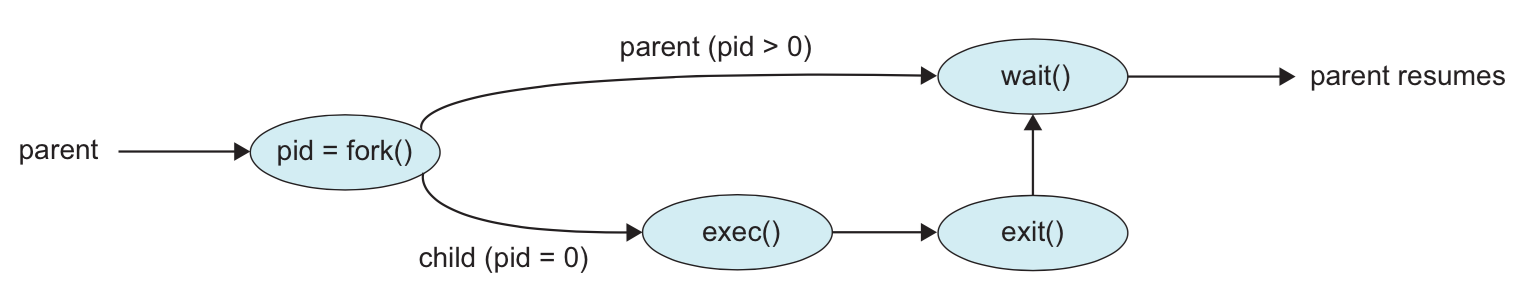
\includegraphics[width=0.85\textwidth]{images/fork-syscall.png}\\
Process creation with the \texttt{fork} system call~\cite{osc}.
\end{center}

What about termination? On the assumption that the process is terminating normally and not being killed, the system call for that is \texttt{exit}. Let us modify that code above to fork off a child process that will exit ``abnormally'' with an exit code of 1. The \texttt{wait} function also returns the process ID of the child so that the parent can identify which of its children has terminated, though it is not used in this example.


\begin{verbatim}
#include <sys/types.h>
#include <stdio.h> 
#include <unistd.h>

int main()
{
  pid_t pid;
  int childStatus;

  /* fork a child process */
  pid = fork();
  
  if (pid < 0) { 
  
    /* error occurred */ 
    fprintf(stderr, "Fork Failed"); 
    return 1;
    
 } else if (pid == 0) { 
    
    /* child process */
    exit( 1 );
    
  } else { 
    
    /* parent process */
    /* parent will wait for the child to complete */
    wait(&childStatus);
    printf("Child Complete with status: %i \n", childStatus);
    
  }
    
  return 0;
}
\end{verbatim}

If the program itself has no explicit call to \texttt{exit}, the \texttt{return} statement at the end of \texttt{main} will have the same effect.

\section*{UNIX System V Process Management}

UNIX divides its processes into two categories: system processes that run in kernel mode and user processes that run in user mode. There are nine different states a process can be in~\cite{osi}.

\begin{enumerate}
	\item \textbf{User Running:} Executing in user mode.
	\item \textbf{Kernel Running:} Executing in kernel mode.
	\item \textbf{Ready to Run, in Memory:} Ready to run; in memory.
	\item \textbf{Asleep in Memory:} Blocked; in memory.
	\item \textbf{Ready to Run, Swapped:} Ready to run; not in memory.
	\item \textbf{Sleeping, Swapped:} Blocked; not in memory.
	\item \textbf{Preempted:} Process is returning from kernel to user mode, but the kernel decides to run another process at this time.
	\item \textbf{Created:} Newly created and not yet ready to run.
	\item \textbf{Zombie:} Process is done, but the parent has not yet collected the return information.
\end{enumerate}


\begin{center}
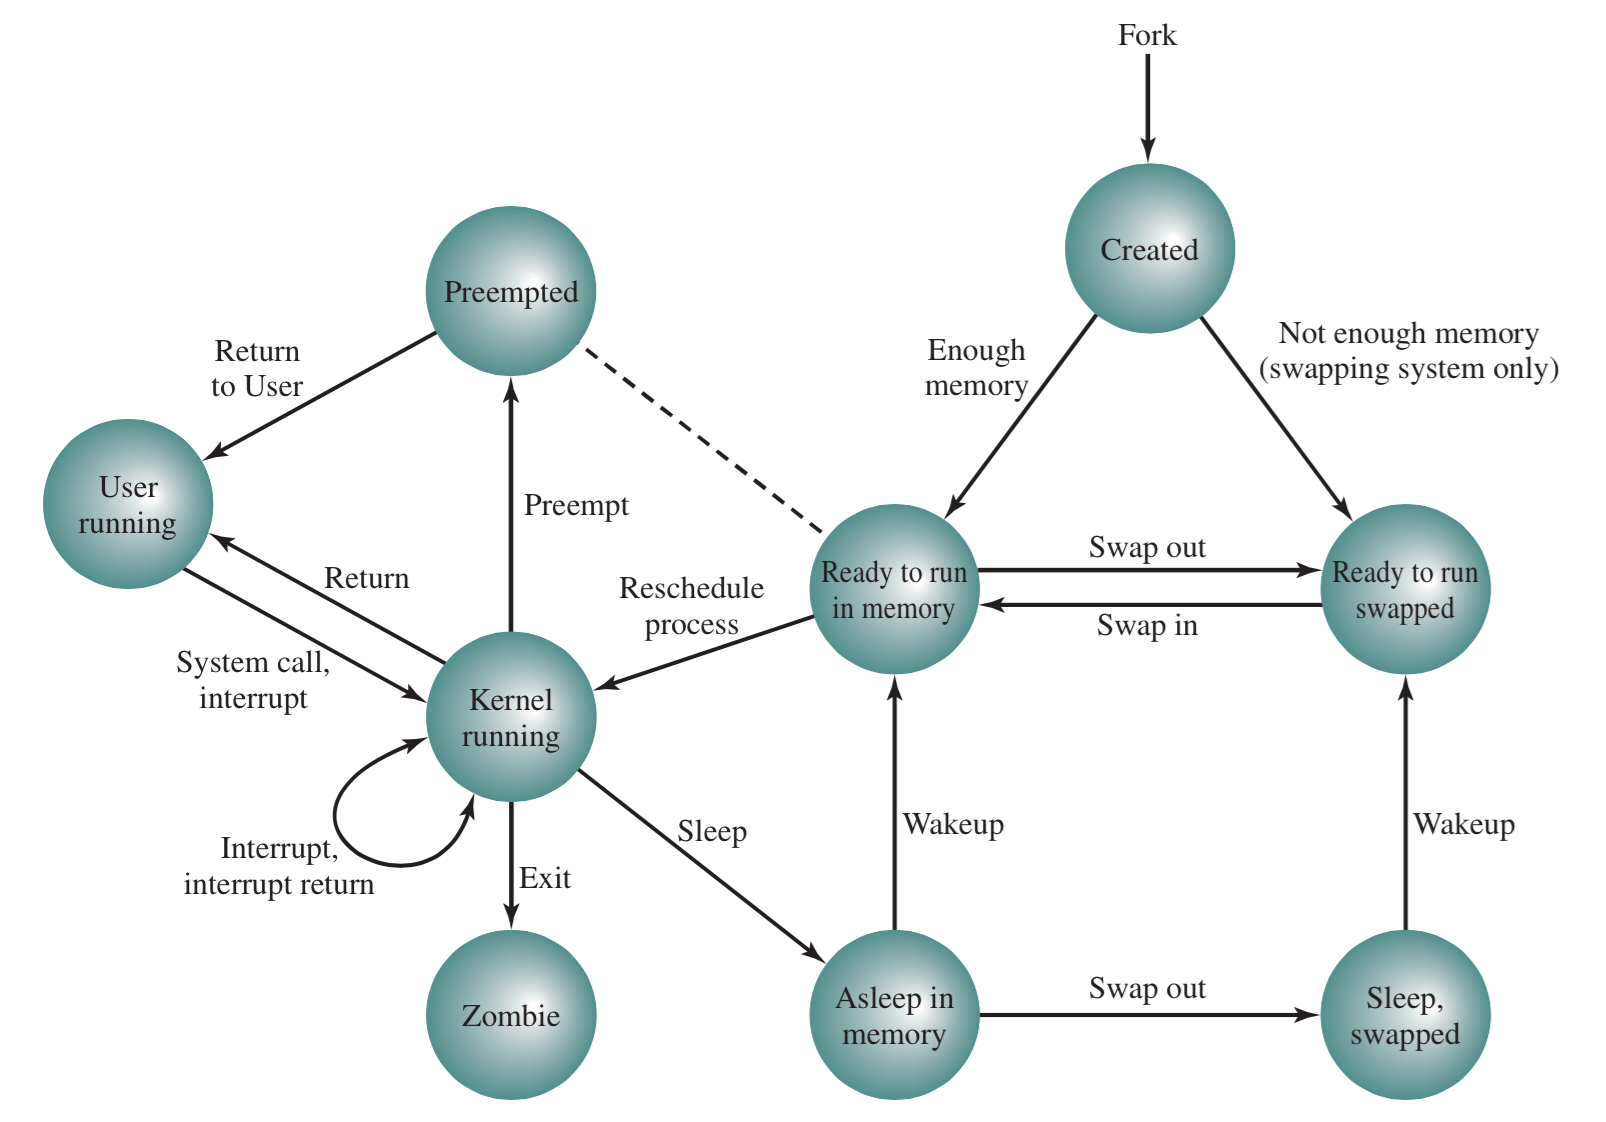
\includegraphics[width=0.75\textwidth]{images/unix-states.png}\\
UNIX process state transition diagram~\cite{osi}.
\end{center}

This is much like our general seven-state model we saw earlier. There are two major differences: (1) the running in user mode vs. running in kernel mode distinction; and (2) the preempted state. This preempted state is just like ready to run in memory, but the distinction is really just how the process got to be in that state. When a process is running in kernel mode as a result of a system call, for example, when control is about to go back to the user program, this is as good a time as any to swap to another process. So that would put the process in the preempted state rather than ready to run, in memory. But these two states are really the same, logically~\cite{osi}. 

\subsection*{Process Creation}
Process creation, as already discussed, takes place when \texttt{fork} is called. When that happens, the OS takes the following steps~\cite{bach86}:

\begin{enumerate}
	\item It allocates a slot in the process table for the new process.
	\item It assigns a unique process ID to the child process.
	\item It makes a copy of the process image of the parent, with the exception of any shared memory.
	\item It increments counters for any files owned by the parent (showing there is an additional process referencing those files).
	\item The new process is in the state Ready to Run.
	\item A return value of 0 goes to the child process, and the unique process ID of the child is returned to the parent.
\end{enumerate}

All of the above takes place in kernel mode in the parent process. When it is all done, the system will need to choose which process is going to run: 

\begin{enumerate}
	\item The parent process. The child is in the ready to run state.
	\item The child process. The parent is in the ready to run state.
	\item Another process. Both parent and child are in the ready to run state.
\end{enumerate}

It may seem a little strange that to spawn a process, the parent must first make a clone of itself and continue from the same point, branching only if the return value of the ID is tested.

\section*{The Fork Bomb}

We will take a slight digression from the general topic of processes to discuss a denial-of-service attack against UNIX systems that is called the ``Fork Bomb''. The idea behind the attack is to call \texttt{fork} repeatedly until the number of processes spawned is too high for the system to manage and it either crashes or is so slow that no useful work can get done. As you can imagine, this is caused by repeatedly calling \texttt{fork}. Each time a program does so, there are now two processes running, each of which calls \texttt{fork}. There are then $2^{n}$ processes after each of $n$ invocations and this exponential growth will soon crash up against the limits of the system.

A system configured to defend against this may impose limits on (1) the total number of processes a user may create; and (2) the rate at which a user may spawn a new process.

Note: do not attempt this on anything other than your personal computer at home. It is a denial of service attack and would certainly count as misuse of resources on any system. Accordingly, trying to do it will very likely result in a ban. Getting banned from using university computer resources is not conducive to completing your degree.

\bibliographystyle{alphaurl}
\bibliography{252}


\end{document}